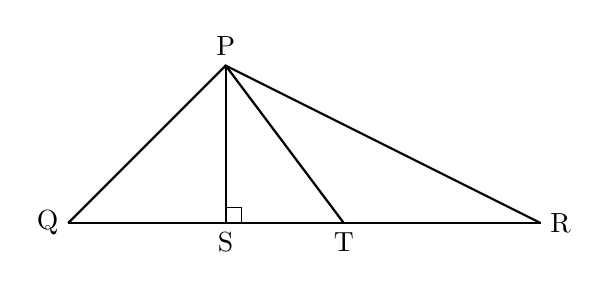
\begin{tikzpicture}[scale=1]
% Base line
\draw[thick] (0,0) coordinate (Q) -- (6,0) coordinate (R);
% Point P and Altitude PS
\coordinate (S) at (2,0);
\coordinate (P) at (2,2);
\draw[thick] (Q) -- (P) -- (R);
\draw[thick] (P) -- (S);
% Point T
\coordinate (T) at (3.5,0);
\draw[thick] (P) -- (T);
% Labels
\node[left] at (Q) {Q};
\node[below] at (S) {S};
\node[below] at (T) {T};
\node[right] at (R) {R};
\node[above] at (P) {P};
% Right angle symbol
\draw (2,0.2) -- (2.2,0.2) -- (2.2,0);
\end{tikzpicture}